\documentclass[svgnames]{beamer}
%\documentclass[svgnames, handout]{beamer}

\usetheme{i4}

\setbeamertemplate{navigation symbols}{}

\usepackage{setspace}
\usepackage{graphicx}
\usepackage{color}
\usepackage{subfigure}
\usepackage{listings}
\usepackage{amsmath}
\usepackage{amssymb}

\usepackage{textpos}

\usepackage{rotating}
\usepackage{xcolor}
\usepackage{colortbl}

\usepackage{gnuplottex}

\usepackage{gnuplot-lua-tikz}
\definecolor{i4red}{rgb}{0.69,0.11,0.18}
\definecolor{i4blue}{rgb}{0.0,0.4,0.62}
\definecolor{i4green}{rgb}{0.0,0.62,0.4}
\definecolor{i4gray}{rgb}{0.827,0.827,0.827}
\definecolor{darkred}{rgb}{0.8,0,0}
\definecolor{myblue}{rgb}{0,0.1,0.6}
\definecolor{myheadblue}{rgb}{0,0.2,0.7}
\definecolor{myred}{rgb}{0.63,.16,.16}
\definecolor{lstshade}{gray}{0.95}
\definecolor{lstframe}{gray}{0.80}
\definecolor{lstcomment}{gray}{0.5}
\definecolor{lstattrib}{rgb}{0,0.34,0}
\definecolor{remark}{rgb}{1.0, 0.9, 0.9}
\definecolor{remarkframe}{rgb}{1.0, 0.7, 0.7}
\definecolor{i4red}{rgb}{0.69,0.11,0.18}
\definecolor{color_c}{rgb}{0.1686,0.5373,0.8431}
\colorlet{lavender}{blue!60!black!20}
\colorlet{darklavender}{blue!60!black!60}
\colorlet{beige}{yellow!70!black!50!white}
\colorlet{c1blue}{color_c!70!white}

%\setlength{\tabcolsep}{8pt}
%\renewcommand{\arraystretch}{1.5}
%
%\setbeamertemplate{section in toc}{%
%    \color{i4red} $\bullet$  \color{i4blue} \inserttocsection \par}
%
%\setbeamertemplate{subsection in toc}{
%    \color{i4red} \quad $\hookrightarrow$ \color{i4blue} \inserttocsubsection \par}


\institute{Friedrich-Alexander Universit\"at Erlangen-N\"urnberg}
\title[Vergleich nichtblockierender Queues]{Praktikum angewandte Systemsoftwaretechnik: \\
Vergleich nichtblockierender Queues} 

\author{Michael Banken \and Lorenz Haspel} % Your name

\date{9.9.2013} % Date, can be changed to a custom date


\begin{document}


\begin{frame}

	\titlepage
\end{frame}

\begin{frame}
\frametitle{empty}
\begin{itemize}
\item empty
\end{itemize}
\end{frame}

%-----------------------------------------
\begin{frame}
\frametitle{Ergebnisse}


\begin {figure}
      \begin{center}
	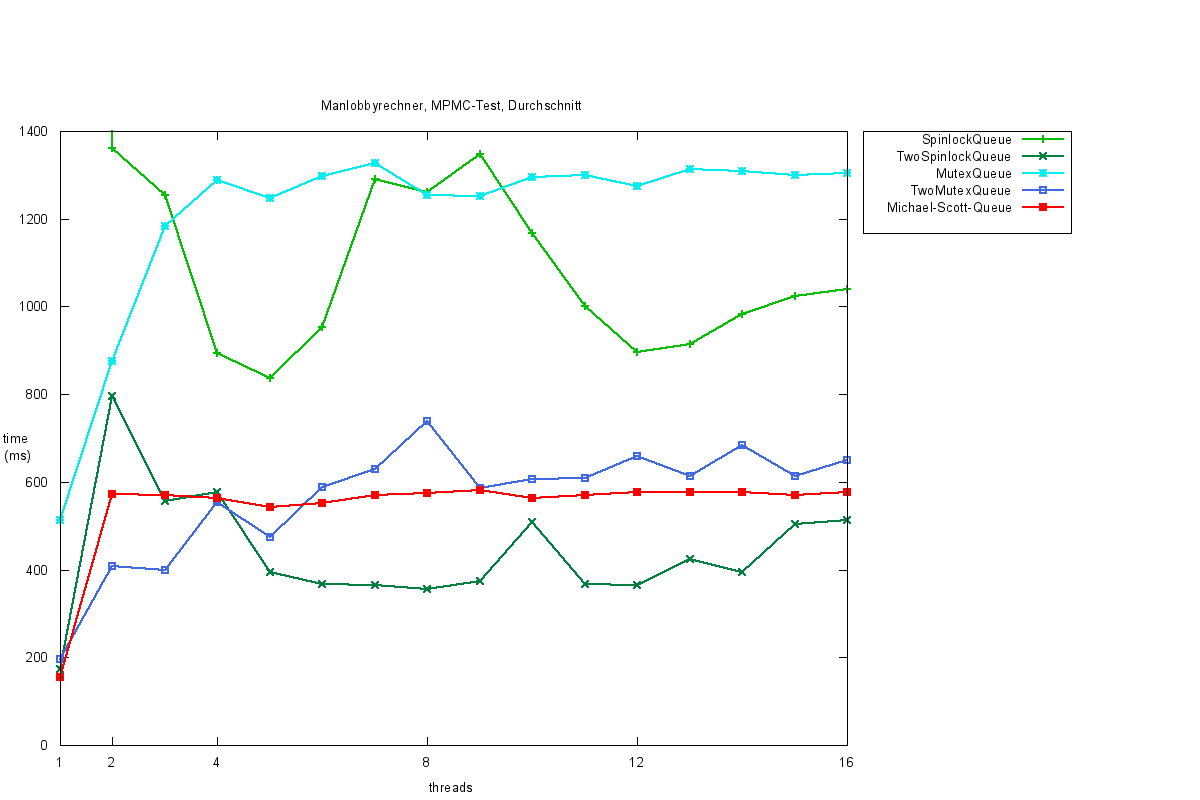
\includegraphics[width=\textwidth]{manma.png}
     \end{center}
\end {figure}
\end{frame}

%-----------------------------------------
\begin{frame}
\frametitle{Ergebnisse}


\begin {figure}
      \begin{center}
	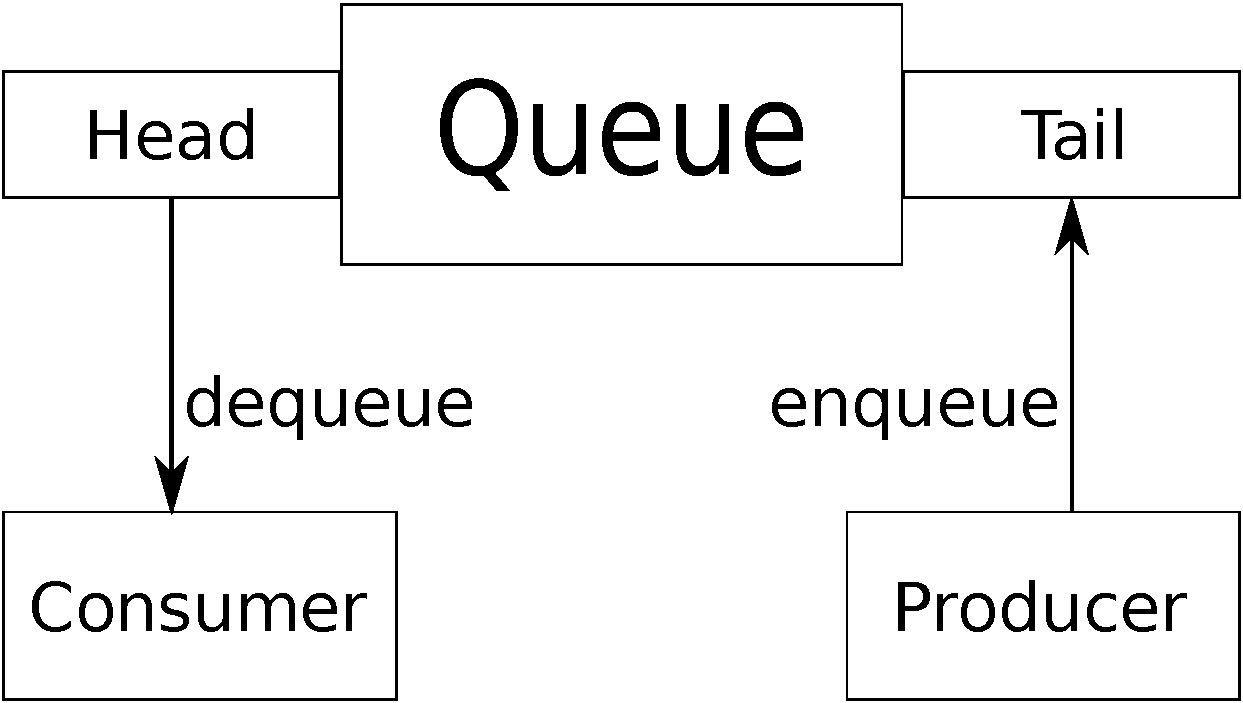
\includegraphics[width=\textwidth]{mpmc.pdf}
     \end{center}
\end {figure}
\end{frame}


%-----------------------------------------

%-----------------------------------------
\begin{frame}
\frametitle{Fazit}
\begin{itemize}
\item empty
\end{itemize}
\end{frame}


%------------------------------------------------
\begin{frame}
\Large{\centerline{Vielen Dank f\"ur Ihre Aufmerksamkeit!}}
\end{frame}



\end{document}
